\documentclass[10pt,a4paper]{article}
\usepackage[utf8]{inputenc}
\usepackage[spanish]{babel}
\usepackage{amsmath}
\usepackage{amsfonts}
\usepackage{amssymb}
\usepackage{makeidx}
\usepackage{graphicx}
\usepackage{lmodern}
\usepackage{kpfonts}
\usepackage{fourier}
\usepackage[hidelinks]{hyperref}
\usepackage[left=2cm,right=2cm,top=2cm,bottom=2cm]{geometry}
\title{Línea de Empaquetado de Arroz.}
\author{Alvarez Sotelo Gabriel\\Mejorada Lopez Ivan\\Torres Pinto Luis Angel\\Vargas Diaz Marco Antonio}
\\
\begin{document}
\maketitle
\centering

\includegraphics[scale=1.90]{upzmg.jpg}\\ 
\raggedright
\newpage
\section{Introducción.}
La línea de producción surgió en la Revolución Industrial (S. XVIII – XX) como forma de organización de la producción en la que cada trabajador se especializaba en una función específica y manejaba máquinas, también mejor desarrolladas tecnológicamente, elevando la calidad de los productos y los tiempos de producción por unidad. La producción era mayoritariamente artesanal. La creciente demanda de productos, la existencia de un capital cuantioso derivado de un floreciente comercio y la abundancia de una mano de obra barata, fueron los factores que motivaron la innovación de herramientas y maquinarias utilizables en el diseño de nuevos procesos productivos que fueran capaces de satisfacer la demanda existente. 
Desde que surgió la revolución industrial no falto poco tiempo para que maquinaria especializada reemplazara al trabajador, reduciendo costos y tiempos de producción, el cual resulto mas eficaz.\\ 
Las líneas de producción han evolucionado para optimizar los procesos a eto se le llama automatización. Esto ha permitido disminuir errores, tiempos y mejorar la calidad final del producto. Reducir costes y aumentar la eficiencia son otras ventajas de dicha evolución. 
\\
\section{Planteamiento del problema.}
Las línea de producción convencionales tienen el problema de que son muy costosas y el tiempo de producción es muy elevado, para la industria resulta un grave problema ya que a ella entre menos sea el tiempo en que produce un producto resulta mas eficaz, por ello nosotros solucionaremos mediante una línea de producción automatizada la cual tendra un tiempo de producción menor a una convencional.  
\\
\section{Objetivo general del proyecto.}
Medir el tiempo en el cual producirá nuestra línea de producción, y verificar que nuestra linea de producción sea menos costosa.
Demostrando que nuestra línea de producción es mas eficaz que una convencional. Para ello tendremos que proponer, diseñar, evaluar y elaborar mejores procesos a nuestra línea de producción para así poder medir el tiempo y determinar que la nuestra es mejor. 
\section{Objetivos del proyecto.}
1.Que el proyecto sea menos costoso de lo ya cotizado.
2.Correr nuestra línea de producción.
3.Verificar que tenga mejor tiempo de producción.
4.Determinar que el proyecto sea mas eficaz y tenga un mejor rendimiento en cuanto a calidad del producto. 
\\
\section{Justificación}
Decidimos escoger dicho tema ya que para nosotros es importante brindar una solución para que las líneas de producción tengan menores costos y el resultado del tiempo de producción sea el menor posible así como también tenga mejor calidad el producto final.
Queremos demostrar que las lineas de produccion se pueden automatizar mejor y tener mejores tiempos, costos y calidad. Es por ello que decimos optar por el tema de las líneas de producción ya que es de nuestro agrado y nos importa mejorar el entorno de la industria y poder llegar a mejorarla aun más. 
\\ 
\section{Delimitación.}
Situcacion actual: en la situcaion actual estamos investigando las etapas de una línea de producción, desde como se utiliza como se programa también vemos sus costos, la historia y en que se puede llegar a beneficiar a nosotros como sociedad.

Tenemos bajo presumuesto y algunos materiales que ocupamos, estan un poco dificiles de conseguir, tenemos poco tiempo y también tenemos falta de conocimiento del tema para poder concluirlo.
\\
\section{Posibles materiales y Costos.}
\centering
\begin{tabular}{|c|c|}\hline
Materiales & Costo \\\hline
Electroválvula & \$200 \\ \hline
Motor de dos sensores de presencia & \$50 \\ \hline
Plc & \$900 \\ \hline
Banda & \$380 \\ \hline
Tabla & \$250 \\ \hline
Botones & \$60 \\ \hline
Bisagras & \$120 \\ \hline
Soportes & \$200 \\ \hline
Caja de acrílico & \$200 \\ \hline
Cervomotor & \$100 \\ \hline
Material que se necesita para dispersar(Arroz) & \$40 \\ \hline
Total & \$2500 \\ \hline

\end{tabular}\\
\raggedright
\section{Matriz de Roles.}
Luis Angel Torres Pinto: Recolección del dinero para comprar los componentes, la segunda tarea que tendré será hacer un check list de los materiales con los que contamos, tambien tendré de tarea hacer cada uno de los bocetos y cálculos que se necesitan para lograr el funcionamiento.\\
Ivan Mejorada Lopez : Seré el encargado de verificar si los diagramas y cálculos están correctos, también ayudare con el armado y programación del plc, revisare conexiones y todo el montaje de el mismo proyecto.\\
Gabriel Alvarez Sotelo: Me encargare de concectar todo como viene en el diagrama, ayudar con el montaje del plc, y configurar los sensores que llevara el proyecto, al finalizar revisare que todas las conexiones sean correctas y adecuadas para poder utilizarlo. \\
Marco Antonio Vargas Diaz: Yo apoyare en todos los facotres desde la recolección del dinero, hasta comprar cada uno de los materiales, ayudare en la parte de la programación, y el diseño que le dará forma a nuestro proyecto.
\\
\section{Diagrama Gantt de tiempos y actividades.}\\
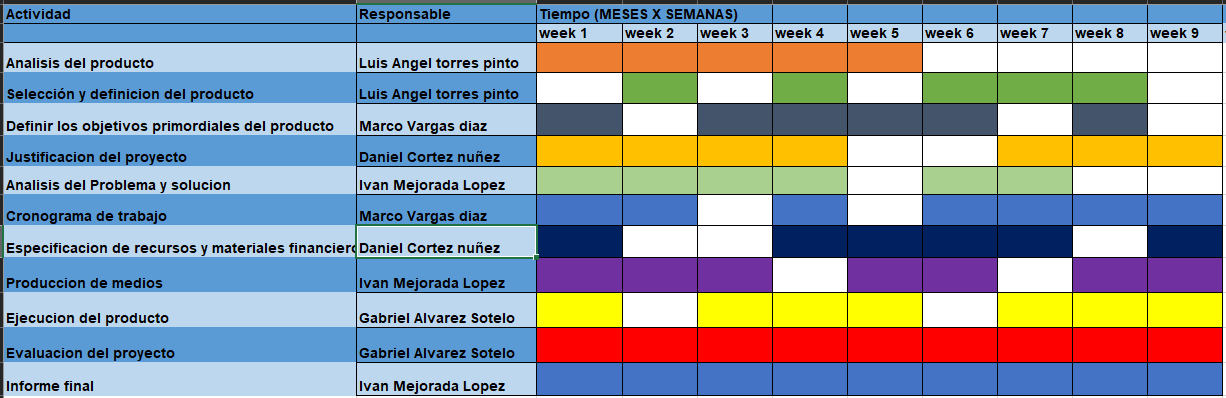
\includegraphics[scale=.42]{gantt.png} 
\\
\centering
\section{Aportación de cada materia cursada en el cuatrimestre al proyecto.}
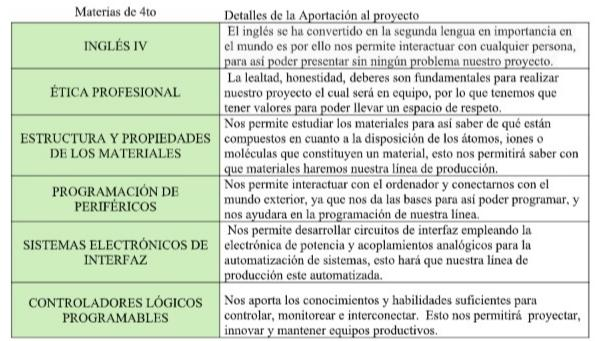
\includegraphics[scale=.68]{tabla.jpeg} \\
\raggedright
\bigskip 
Ingles IV: Esta materia nos ha aportado hasta el momento vocabulario sobre el idioma ingles, así mismo nos permite dominar, hablar, escribir. Esto favorece a nuestro proyecto, ya que podemos presentarlo en otro idioma además del español, para así poder comunicarnos con nuestra audiencia.\\

Ética profesional: Esta materia nos orienta al análisis, la reflexión lo cual nos permitirán tomar conciencia sobre nuestro desempeño personal, social y laboral. Aprender a colaborar con nuestro equipo así mismo actuar en el ámbito personal, social y laboral desde una perspectiva ética y ciudadana.\\

Estructura y Propiedades de los materiales: La materia nos ha aportado hasta el momento los criterios para buscar y seleccionar los materiales apropiados para nuestras aplicaciones.  Lo cual para ello es necesario comprender como están constituidos los materiales y así establecer el tipo de propiedades que tiene dicho material para poder determinar que tipo de aplicación le daremos.\\

Programación de periféricos: Ha aportado la capacidad para comprender el proceso de transferencia de datos a través de puertos estándar e inalámbricos, para asi realizar la comunicación de datos y el diseño de interfaces de hardware y software.\\

Sistemas electrónicos de interfaz: Ha aportado comprender y analizar sistemas de automatización con base en el diagnóstico del proceso, mediante procedimientos de interconexión y acoplamiento. Nos ha permitido diagnosticar operaciones y procesos susceptibles a automatizar mediante el análisis del proceso. \\

Controladores Lógicos Programables: Nos aporta los conocimientos para controlar, monitorear e interconectar con un PLC, y nos brinda la capacidad de aplicar los conocimientos en la práctica.
\section{Desarrollo del proyecto.}
Este proyecto se llevará a cabo mediante etapas las cuales serán de acuerdo a lo que vallamos observando en la construcción de nuestra línea de producción, desde la compra de los materiales, la programación del plc, el diseño de la línea de producción. Para ello tendremos que adquirir las bases de como realmente funciona desde adentro una linea de produccion y con base a eso desarrollar la idea, para nosotros es importante esto ya que no queremos dejar una idea ya empezada. 
\\
\section{Bibliografía.}
S.L,I.(4 de 6 de 2019). Infaimon. Obtenido de INFAIMON:                           

\url{https://blog.infaimon.com/la-linea-produccion/}\\
\bigskip 
Andrea.(19 de 07 de 2019).Educativos.Obtenido de Educativos:\url{https://www.educadictos.com/aparicion-de-la-produccion-en-serie/}\\
\bigskip
Villagran, A.C.(7 de 02 de 2011). slideshare. Obtenido de slideshare: 
\url{https://es.slideshare.net/castrov/historia-de-la-produccin}

\end{document}
\end{document}